\documentclass[conference]{IEEEtran}
\IEEEoverridecommandlockouts

% Các gói chuẩn theo mẫu hội nghị IEEE.
\usepackage{cite}
\usepackage{amsmath,amssymb,amsfonts}
\usepackage{algorithmic}
\usepackage{graphicx}
\usepackage{textcomp}
\usepackage{xcolor}
\usepackage[utf8]{inputenc}
\usepackage[T5]{fontenc}

% Các gói bổ sung cần thiết cho nội dung bài báo.
\usepackage{bm}
\usepackage{booktabs}
\usepackage{multirow}
\usepackage{array}
\usepackage{url}
\graphicspath{{images/}}

% Allow up to 3 floats at the top of a column (default is 2).
\setcounter{topnumber}{3}
\renewcommand{\topfraction}{0.92}

\def\BibTeX{{\rm B\kern-.05em{\sc i\kern-.025em b}\kern-.08em
    T\kern-.1667em\lower.7ex\hbox{E}\kern-.125emX}}

% Cho phép ngắt hàng giữa các nhóm tác giả trong chế độ conference.
\makeatletter
\newcommand{\linebreakand}{%
  \end{@IEEEauthorhalign}
  \hfill\mbox{}\par
  \mbox{}\hfill\begin{@IEEEauthorhalign}}
\makeatother

% ============================================================
\begin{document}
\pagestyle{plain}

\title{HBCC: Hybrid Block Context Cluster cho phân loại ảnh nhẹ}

\author{
\IEEEauthorblockN{Nguyễn Việt Hùng}
\IEEEauthorblockA{\textit{Khoa Công nghệ Thông tin} \\
\textit{Trường Đại học Khoa học Tự nhiên,} \\
\textit{Đại học Quốc gia Thành phố Hồ Chí Minh} \\
Thành phố Hồ Chí Minh, Việt Nam \\
23122032@student.hcmus.edu.vn}
\and
\IEEEauthorblockN{Nguyễn Bá Nam}
\IEEEauthorblockA{\textit{Khoa Công nghệ Thông tin} \\
\textit{Trường Đại học Khoa học Tự nhiên,} \\
\textit{Đại học Quốc gia Thành phố Hồ Chí Minh} \\
Thành phố Hồ Chí Minh, Việt Nam \\
23122043@student.hcmus.edu.vn}
\linebreakand
\IEEEauthorblockN{Lê Hoàng Thái$^{*}$\thanks{$^{*}$Tác giả liên hệ.}}
\IEEEauthorblockA{\textit{Khoa Công nghệ Thông tin} \\
\textit{Trường Đại học Khoa học Tự nhiên,} \\
\textit{Đại học Quốc gia Thành phố Hồ Chí Minh} \\
Thành phố Hồ Chí Minh, Việt Nam \\
lhthai@fit.hcmus.edu.vn}
}

\maketitle

% ============================================================
\begin{abstract}
Phân loại ảnh trên thiết bị biên đòi hỏi sự cân bằng giữa độ chính xác
và chi phí tính toán. Các CNN nhẹ giảm chi phí nhưng có thể hạn chế
khả năng biểu diễn, trong khi Context Cluster (CoC) tổng hợp ngữ cảnh
bằng phân cụm nhưng bỏ qua kết cấu cục bộ và có nguy cơ suy biến token
trên ảnh nhỏ. Bài báo đề xuất \textbf{HBCC} (\textit{Hybrid Block
Context Cluster}), kiến trúc lai bốn tầng sử dụng LBPConv và DWConv ở
độ phân giải cao, sau đó chuyển sang phân cụm thuần. Thiết kế stem,
độ sâu từng tầng và fold partitioning được điều chỉnh để hạn chế suy biến
token; chưng cất tri thức từ ResNet-18 được dùng để hỗ trợ huấn luyện.
Trên CIFAR-10, HBCC-Medium+KD đạt \textbf{95,36\%} top-1 với 1,76M
tham số và 138,8M MACs. Trên Food-101 ở độ phân giải
$224\!\times\!224$, biến thể HBCC-2.5M huấn luyện từ đầu đạt
\textbf{82,53\%} top-1 và \textbf{95,33\%} top-5; mô hình chỉ kém
ResNet-18 lần lượt 0,38\% và 0,16\% trong khi sử dụng ít
tham số hơn \textbf{4,38} lần. Trên Tiny-ImageNet-200 (200 lớp),
HBCC-Medium+KD đạt \textbf{58,90\%}, vượt cả ResNet-18 giáo viên
(58,58\%) với 6,26 lần ít tham số hơn. Phân tích toán tử cho thấy
sự phân mảnh kernel vẫn là nút thắt khiến mức giảm MACs chưa chuyển
hóa hoàn toàn thành cải thiện độ trễ thực đo.
\end{abstract}

\begin{IEEEkeywords}
Phân loại ảnh, Context Cluster, kiến trúc lai cục bộ--phân cụm,
mạng nơ-ron nhẹ, chưng cất tri thức.
\end{IEEEkeywords}

% ============================================================
\section{Giới thiệu}
\label{sec:intro}

Phân loại ảnh trên thiết bị biên đòi hỏi sự cân bằng giữa độ chính xác
và chi phí tính toán. Các mô hình CNN sâu~\cite{He2016ResNet} và Vision
Transformer~\cite{Dosovitskiy2021ViT} có khả năng biểu diễn mạnh nhưng
thường vượt quá giới hạn tài nguyên của nền tảng nhúng.
MobileNetV2~\cite{Sandler2018MobileNetV2} và
ShuffleNetV2~\cite{Ma2018ShuffleNetV2} giảm chi phí tính toán, song
việc tinh giản kiến trúc có thể hạn chế khả năng biểu diễn đặc trưng.

Context Cluster (CoC)~\cite{Ma2023ImageAsSetOfPoints} cung cấp một
hướng tiếp cận khác bằng cách biểu diễn ảnh như tập hợp điểm và tổng
hợp ngữ cảnh thông qua phân cụm. Tuy nhiên, phân cụm thuần túy bỏ qua
kết cấu cục bộ ở độ phân giải cao. Trên ảnh nhỏ, việc giảm độ phân giải
quá nhanh còn có thể gây \emph{suy biến token}, khiến số điểm trong mỗi
cụm không đủ để phép tổng hợp ngữ cảnh phát huy tác dụng.

Nghiên cứu này hướng tới xây dựng một kiến trúc nhẹ kết hợp xử lý cục
bộ với phân cụm ngữ cảnh, đồng thời khảo sát cách phân bổ hai cơ chế
theo độ phân giải. Nghiên cứu đánh giá cả ảnh nhỏ
($32\!\times\!32$) và ảnh độ phân giải chuẩn
($224\!\times\!224$), với ngân sách không quá 3M tham số cho HBCC,
thông qua hai câu hỏi:

\noindent\textbf{(CQ1)} Liệu kiến trúc lai kết hợp xử lý cục bộ và phân cụm ngữ cảnh có thể cải thiện đồng thời độ chính xác và hiệu quả tính toán so với cả CNN nhẹ thuần túy lẫn mô hình thuần phân cụm?

\noindent\textbf{(CQ2)} Chiến lược phân bổ nhánh cục bộ, fold và độ rộng theo tầng có còn hiệu quả khi chuyển từ ảnh nhỏ $32\!\times\!32$ sang đầu vào $224\!\times\!224$ hay không?

Để trả lời các câu hỏi trên, bài báo đề xuất \textbf{HBCC}
(\textit{Hybrid Block Context Cluster}), kiến trúc bốn tầng sử
dụng khối lai ở các tầng có độ phân giải cao và phân cụm thuần ở các
tầng sau. Thiết kế stem và độ sâu từng tầng được điều chỉnh để hạn chế
suy biến token; chưng cất tri thức được sử dụng trong huấn luyện mà
không làm tăng chi phí suy luận của mô hình học sinh.
Đối với Food-101, kiến trúc được mở rộng có kiểm soát lên 2,57M tham
số, dùng stem stride~4 và các vùng phân cụm đồng nhất $7\!\times\!7$
để bảo toàn cấu trúc không gian trên đầu vào $224\!\times\!224$.

% ============================================================
\section{Các nghiên cứu liên quan}
\label{sec:related}

\subsection{Mạng CNN và residual learning}

ResNet~\cite{He2016ResNet} giới thiệu residual connection:
$\mathbf{y} = \mathcal{F}(\mathbf{x}) + \mathbf{x}$,
cho phép gradient truyền thẳng qua lớp, ngăn vanishing gradient và
mở ra kỷ nguyên huấn luyện mạng 50--152 lớp. Standard $3\!\times\!3$
convolution với $C_{\mathrm{in}}$ kênh vào, $C_{\mathrm{out}}$ kênh ra,
kernel size $k$ có chi phí tỷ lệ với
$C_{\mathrm{in}}\!\cdot\!k^2\!\cdot\!C_{\mathrm{out}}$, làm ResNet-18
cần 556,7M MACs dù ảnh chỉ $32\!\times\!32$.

MobileNetV2~\cite{Sandler2018MobileNetV2} thay standard conv bằng
depthwise separable conv: tách thành depthwise ($k\!\times\!k$ riêng
cho từng channel, chi phí $C_{\mathrm{in}}\!\cdot\!k^2$) và pointwise
($1\!\times\!1$, chi phí $C_{\mathrm{in}}\!\cdot\!C_{\mathrm{out}}$),
giảm tổng chi phí về $O(C_{\mathrm{in}}(k^2 + C_{\mathrm{out}}))$ --
tiết kiệm xấp xỉ $1/k^2$ lần. ShuffleNetV2~\cite{Ma2018ShuffleNetV2}
chỉ ra rằng FLOPs không tương quan trực tiếp với tốc độ thực đo và
đề xuất bốn nguyên tắc: (i) cân bằng số channel đầu vào/ra; (ii)
tránh group convolution; (iii) tránh phân nhánh kiến trúc; (iv) giảm
element-wise operations. Các kết quả này cho thấy hiệu quả lý thuyết
cần được kiểm chứng thêm bằng độ trễ thực đo trên phần cứng đích.

\subsection{Vision Transformer và MetaFormer}

ViT~\cite{Dosovitskiy2021ViT} chia ảnh thành $n$ patch và áp dụng
multi-head self-attention:
\begin{equation}
  \operatorname{Attn}(Q,K,V) =
  \operatorname{softmax}\!\!\left(\frac{QK^\top}{\sqrt{d_k}}\right)\!V,
  \label{eq:attn}
\end{equation}
với độ phức tạp $O(n^2 d_k)$. Trên ảnh $32\!\times\!32$ với patch
$2\!\times\!2$, $n{=}256$ token; chi phí $O(256^2)$ là quá lớn cho
bài toán lightweight. Trong khi đó, phân cụm với độ phức tạp
$O(n\!\cdot\!K)$ và $K{=}4$ có chi phí trộn token lý thuyết thấp hơn
xấp xỉ $64\!\times$ so với single-head attention. Các kiến trúc
MetaFormer cho thấy cấu trúc hai khối (trộn token + MLP) của
Transformer quan trọng không kém toán tử cụ thể.

\subsection{Context Cluster}

CoC~\cite{Ma2023ImageAsSetOfPoints} biểu diễn ảnh như tập hợp điểm
5D $(R,G,B,x,y)$, tích hợp tọa độ không gian vào đặc trưng. Cluster
centers được tạo tự động qua AdaptiveAvgPool (không tham số học);
điểm được gán cứng vào cluster gần nhất qua cosine similarity với
chi phí $O(N\!\cdot\!M\!\cdot\!D)$. Hạn chế chính: pure clustering ở
mọi tầng bỏ qua thông tin tần số cao (kết cấu vi mô, cạnh), làm
CoC-baseline chỉ đạt 88,34\% trên CIFAR-10. Ngoài ra, suy biến
token xảy ra khi bản đồ đặc trưng quá nhỏ so với số tâm cụm (phân
tích chi tiết ở Mục~\ref{sec:degeneracy}).

\subsection{Local Binary Pattern}

LBP~\cite{Ojala2002LBP} mã hóa kết cấu tại pixel $(x_c,y_c)$:
\begin{equation}
  \operatorname{LBP}_{P,R}(x_c,y_c) =
  \sum_{p=0}^{P-1} s(g_p - g_c)\cdot 2^p, \quad
  s(u) = \begin{cases}1 & u\geq0\\0 & u<0\end{cases},
  \label{eq:lbp}
\end{equation}
trong đó $g_c$ là cường độ pixel trung tâm, $g_p$ là pixel thứ $p$
trên vòng tròn bán kính $R$ với $P$ điểm mẫu đều nhau. Phép tính
chỉ gồm phép trừ và ngưỡng nhị phân -- gần như không tốn MACs.
LBPConv áp dụng công thức này trên từng channel với bộ lọc cố định
(không học tham số tích chập), phù hợp để trích xuất kết cấu vi mô
trên các bản đồ đặc trưng có độ phân giải cao.

\subsection{Chưng cất tri thức}

Hinton và cộng sự~\cite{Hinton2015Distillation} chỉ ra rằng một mô
hình nhỏ (học sinh) học tốt hơn khi bắt chước phân phối xác suất
``mềm'' của một mô hình lớn (giáo viên). Hàm mất mát KD tổ hợp
cross-entropy với nhãn cứng và KL-divergence với đầu ra giáo viên đã
làm mềm bởi nhiệt độ $T$ (chi tiết ở Mục~\ref{ssec:kd_setup}). Phân
phối mềm có thể truyền thêm thông tin về quan hệ liên lớp, đặc biệt
hữu ích trong bài toán phân loại nhiều lớp.

Nhìn chung, CNN nhẹ khai thác tốt tính cục bộ nhưng còn đánh đổi độ
chính xác; self-attention nắm bắt quan hệ toàn cục nhưng có chi phí
bậc hai theo số token; còn CoC giảm độ phức tạp song bỏ qua kết cấu
vi mô và có nguy cơ suy biến token trên ảnh nhỏ. Các nghiên cứu hiện
có chưa làm rõ cách kết hợp xử lý cục bộ với phân cụm ngữ cảnh, cũng
như cách phân bổ hai cơ chế này theo độ phân giải dưới một ngân sách
tham số nghiêm ngặt. Khoảng trống đó là cơ sở cho phương pháp được
đề xuất trong phần tiếp theo.

% ============================================================
\section{Phương pháp đề xuất}
\label{sec:method}

\subsection{Tổng quan pipeline}

Hình~\ref{fig:pipeline} trình bày toàn bộ pipeline. Input ảnh
$\mathbf{I}\in\mathbb{R}^{B\times3\times32\times32}$ được bổ sung
tọa độ (Mục~\ref{ssec:coord}) và đưa qua Stem convolution
(stride~1), tạo feature map $32\!\times\!32\!\times\!C_1$. Bốn tầng
liên tiếp thực hiện phân tích đặc trưng ở độ phân giải giảm dần;
giữa các tầng là PointReducer (convolution $1\!\times\!1$, stride~2)
để downsample và tăng số channel. Cuối cùng, Global Average Pooling
(GAP) và lớp Linear cho ra vector phân loại $C$-chiều
($C{=}10$ hoặc $100$).

\begin{figure*}[h]
  \centering
  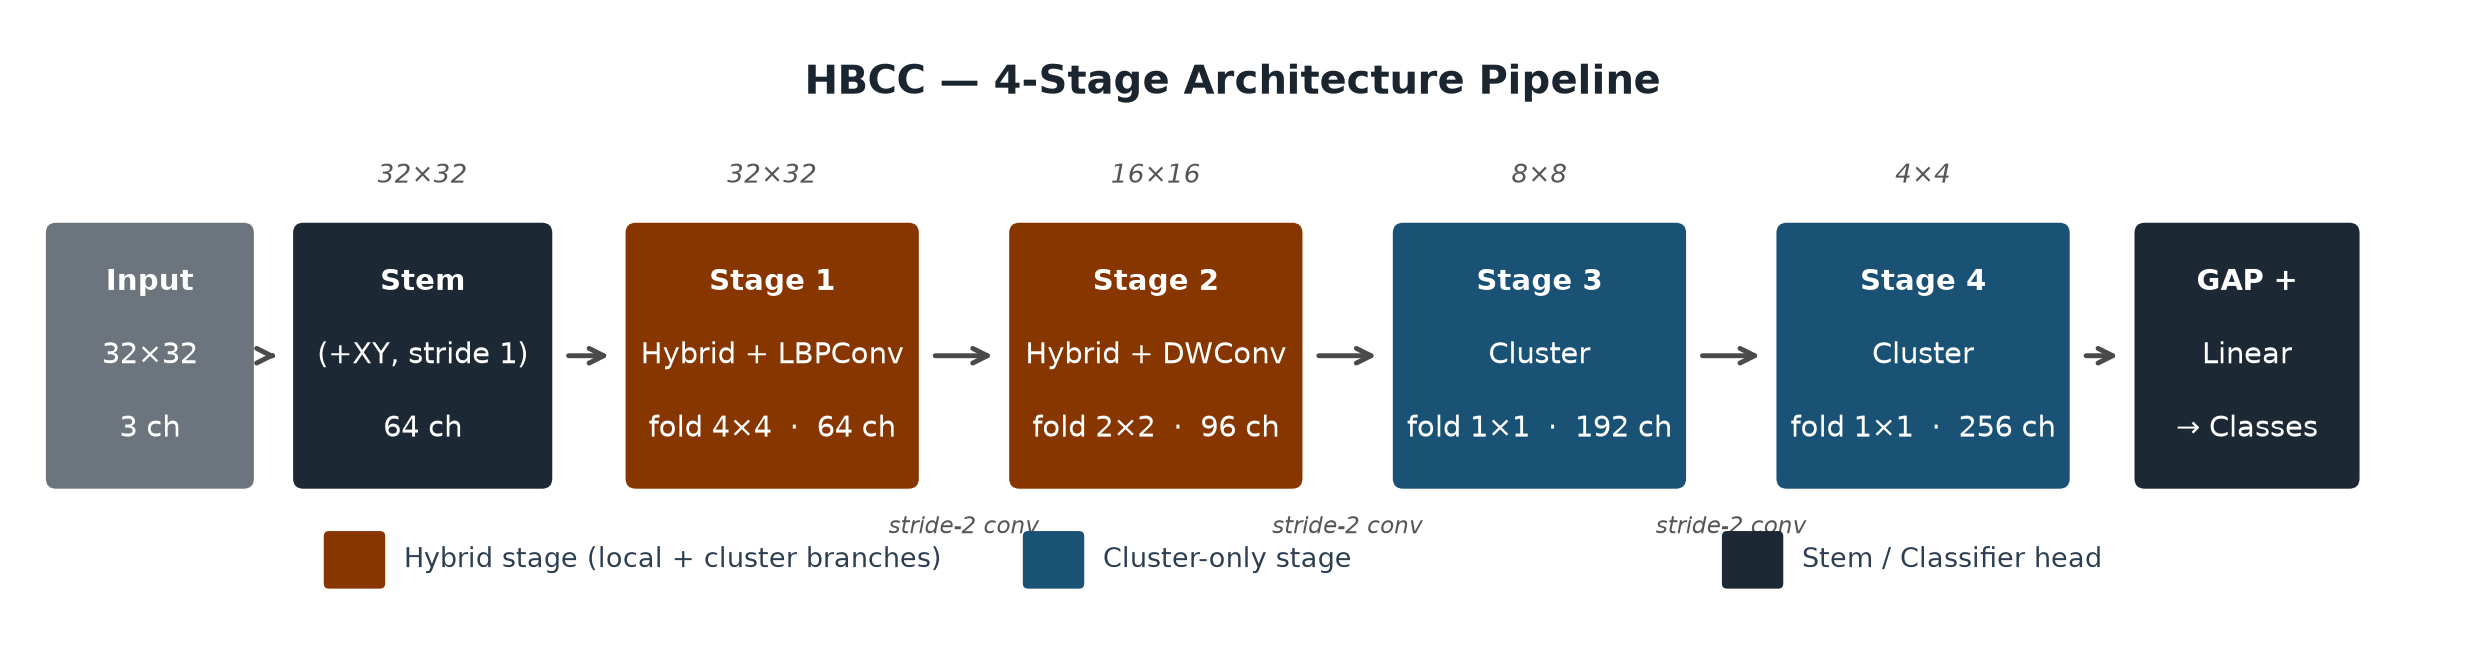
\includegraphics[width=0.97\textwidth]{fig_hbcc_pipeline}
  \caption{Pipeline 4-tầng của HBCC. Màu xanh: Hybrid stage (nhánh
           cục bộ + cluster). Màu đỏ: Cluster-only stage. Độ phân
           giải spatial và số channel $C_i$ ghi chú tại mỗi tầng.}
  \label{fig:pipeline}
\end{figure*}

\subsection{Bổ sung tọa độ $(x,\,y)$}
\label{ssec:coord}

Cosine similarity trên RGB thuần túy không phân biệt hai điểm cùng
màu ở vị trí khác nhau. Chúng tôi bổ sung hai kênh tọa độ chuẩn hóa
về $[0,1]$:
\begin{equation}
  \mathbf{X} = \bigl[\mathbf{I};\;\mathbf{P}_x;\;\mathbf{P}_y\bigr]
  \in\mathbb{R}^{B\times5\times H_0\times W_0},
  \label{eq:coord}
\end{equation}
trong đó $P_x[i,j]=j/(W_0{-}1)$ và $P_y[i,j]=i/(H_0{-}1)$. Bổ
sung tọa độ giúp cluster centers nhận biết vị trí không gian mà
không cần positional encoding tường minh.

\subsection{Cơ chế Context Cluster}
\label{ssec:coc}

Cho feature tensor $\mathbf{X}\in\mathbb{R}^{B\times C\times H\times W}$,
cơ chế này thực hiện sáu bước (trên mỗi head độc lập rồi nối
lại):

\noindent\textbf{Bước 1 -- Chiếu đôi:}
\begin{equation}
  \mathbf{F}=\operatorname{Conv}_{1\times1}(\mathbf{X}),\quad
  \mathbf{V}=\operatorname{Conv}_{1\times1}(\mathbf{X}).
  \label{eq:proj}
\end{equation}
$\mathbf{F}$ dùng để so sánh similarity; $\mathbf{V}$ là giá trị cần
aggregate.

\noindent\textbf{Bước 2 -- Đề xuất cluster centers:}
\begin{equation}
  \mathbf{F}_c = \operatorname{AvgPool}_{K_h\times K_w} \mathbf{F}),\quad \mathbf{V}_c = \operatorname{AvgPool}_{K_h\times K_w}(\mathbf{V}).
  \label{eq:centers}
\end{equation}
Với $(K_h,K_w){=}(2,2)$, mỗi tile cho $K{=}4$ cluster centers.
AdaptiveAvgPool không có tham số học và đảm bảo số centers cố định
bất kể kích thước input.

Lý do chọn \textbf{AvgPool thay vì MaxPool}: tâm cụm phải là
centroid của vùng, không phải cực trị; với LBPConv ở Tầng~1, AvgPool
trên bản đồ nhị phân cho ra histogram mềm phản ánh phân phối kết cấu
trong vùng -- giàu ý nghĩa hơn MaxPool vốn luôn trả về~1 khi bất kỳ
điểm nào được kích hoạt (phân tích chi tiết ở Mục~\ref{ssec:hybrid}).

\noindent\textbf{Bước 3 -- Tính similarity và gán cứng:}
\begin{align}
  s_{ij} &= \sigma\!\left(\alpha\cdot
    \frac{\mathbf{f}_{c_i}\cdot\mathbf{f}_j}
         {\|\mathbf{f}_{c_i}\|\|\mathbf{f}_j\|}+\beta\right),
  \label{eq:sim}\\
  m_{ij} &= \mathbf{1}\!\left[i=\operatorname{arg\,max}_{k}s_{kj}\right],
  \label{eq:mask}
\end{align}
với $\alpha,\beta\in\mathbb{R}$ là tham số học được. Hard assignment
($m_{ij}$) đảm bảo mỗi điểm chỉ đóng góp vào một cluster.

\noindent\textbf{Bước 4 -- Aggregate (trung bình có trọng số):}
\begin{equation}
  \mathbf{g}_i = \frac{\mathbf{v}_{c_i}+\displaystyle\sum_j m_{ij}s_{ij}\mathbf{v}_j} {1+\displaystyle\sum_j m_{ij}s_{ij}}.
  \label{eq:aggregate}
\end{equation}
Mẫu số $1+\displaystyle\sum_j m_{ij}s_{ij}$ chuẩn hóa bao gồm tự-trọng số của center, đảm bảo giá trị đầu ra ổn định kể cả khi cluster rỗng.

\noindent\textbf{Bước 5 -- Dispatch:}
\begin{equation}
  \tilde{\mathbf{v}}_j = \sum_i\mathbf{g}_i\cdot m_{ij}\cdot s_{ij}.
  \label{eq:dispatch}
\end{equation}
Thông tin tổng hợp được phân phối ngược về mỗi điểm theo trọng số.

\noindent\textbf{Bước 6 -- Chiếu đầu ra:}
$\mathbf{Y}=\operatorname{Conv}_{1\times1}(\tilde{\mathbf{V}})$.

\subsection{Fold partitioning}

Ở resolution cao ($32\!\times\!32$, $16\!\times\!16$), phân cụm toàn cục tạo cluster quá lớn, làm mờ chi tiết cục bộ (global over- smoothing). Chúng tôi chia feature map thành $F_h\!\times\!F_w$ tile không chồng lấp:
\begin{equation}
  (B,\,C,\,F_h h,\,F_w w)\;\longrightarrow\;(B F_h F_w,\,C,\,h,\,w).
  \label{eq:fold}
\end{equation}
CoC áp dụng độc lập trong từng tile rồi reshape ngược lại. Fold thu
nhỏ theo tầng: $4\!\times\!4$ (Tầng~1, $32\!\times\!32$),
$2\!\times\!2$ (Tầng~2, $16\!\times\!16$), $1\!\times\!1$
(Tầng~3--4, toàn cục).

\subsection{Hybrid Cluster Block}
\label{ssec:hybrid}

Phân cụm ngữ cảnh và tích chập cục bộ có thế mạnh bổ sung nhau:
phân cụm nắm bắt quan hệ vùng toàn cục nhưng bỏ qua kết cấu vi mô,
trong khi tích chập cục bộ nắm tốt thông tin tần số cao nhưng bị giới
hạn bởi receptive field nhỏ. 

\begin{figure}[!h]
  \centering
  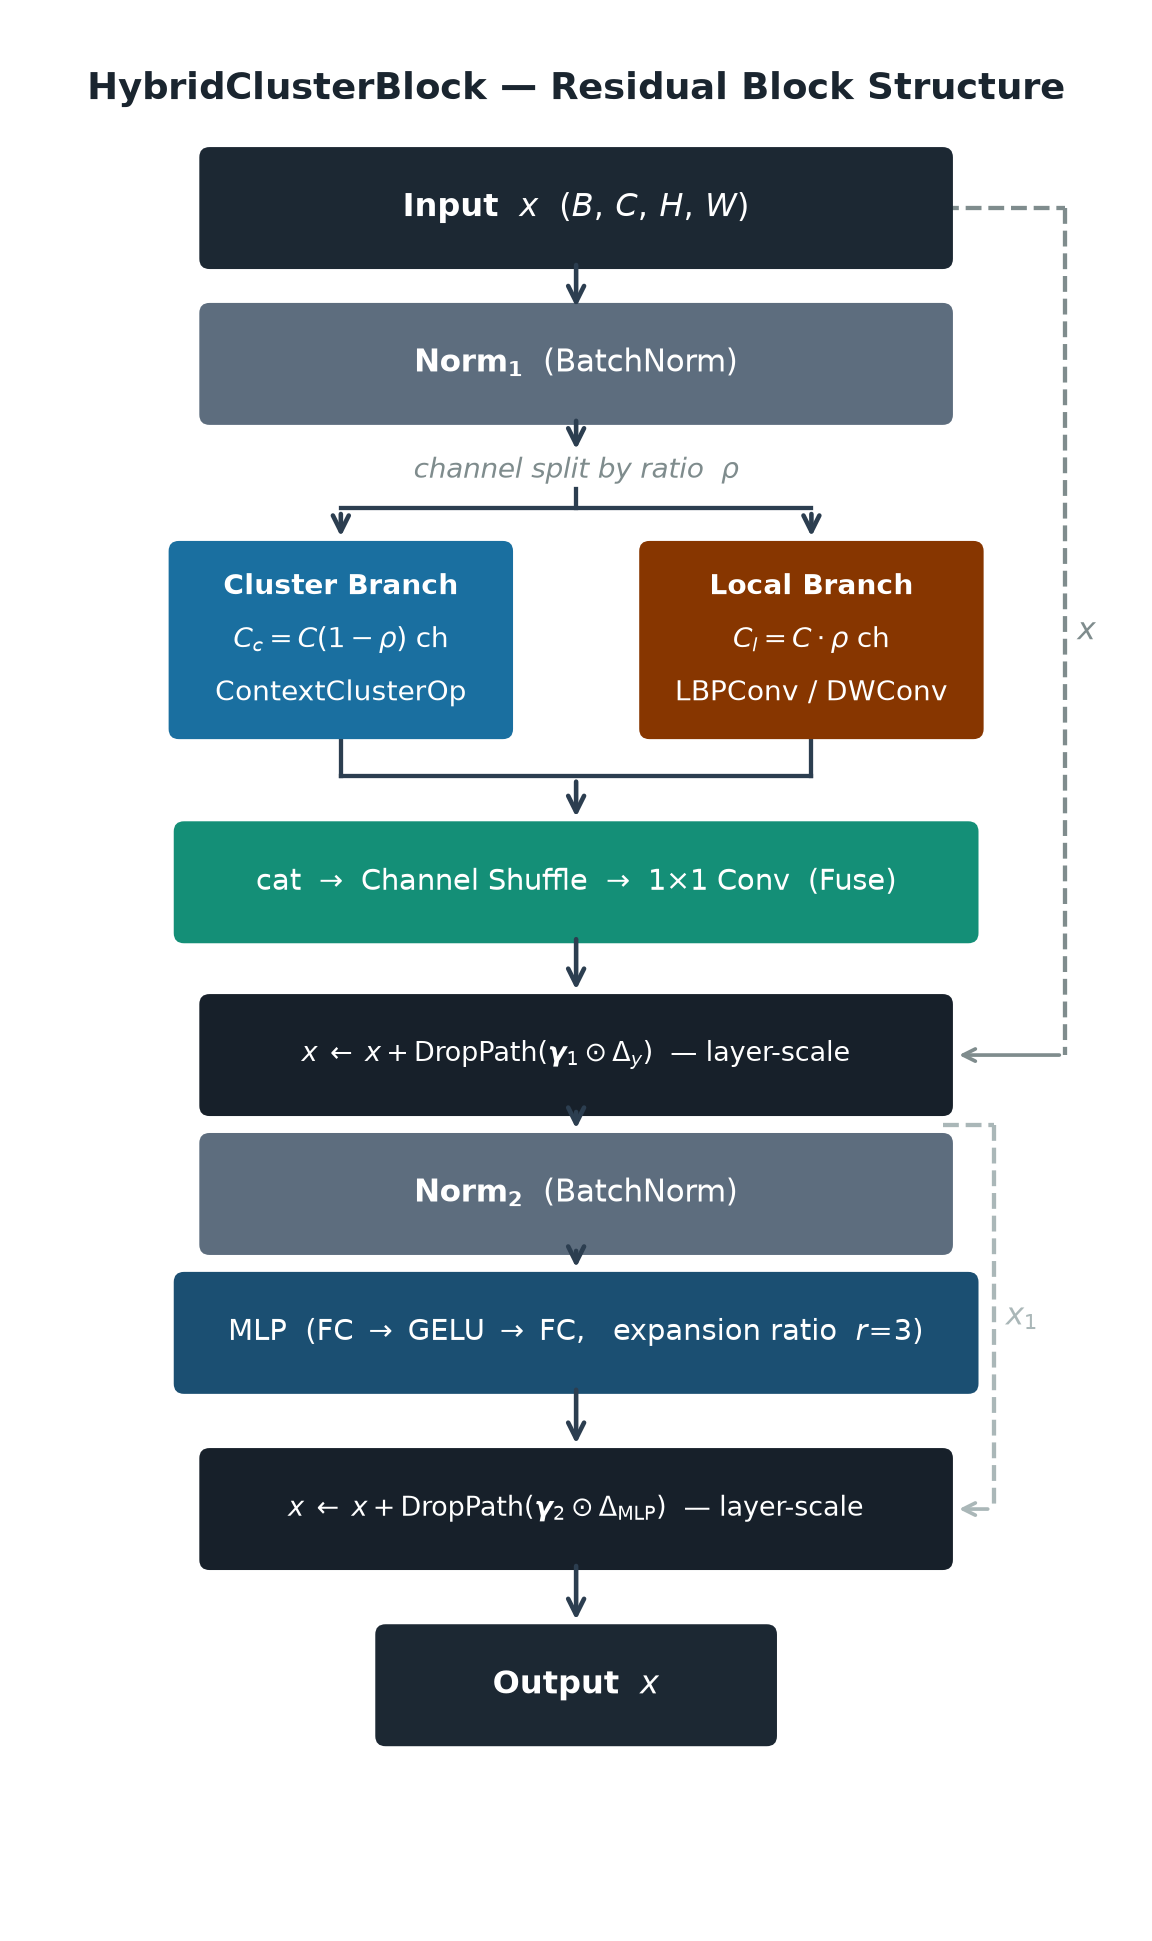
\includegraphics[width=0.95\columnwidth]{fig_hybrid_block}
  \caption{Cấu trúc Hybrid Cluster Block. Nhánh xanh: CoC
           ($C_c{=}C(1{-}\rho)$ channel). Nhánh cam: Local branch
           ($C_l{=}C\rho$ channel). Fuse qua channel shuffle và
           $1\!\times\!1$ conv. Layer-scale $\bm{\gamma}$ khởi
           tạo $10^{-5}$.}
  \label{fig:hybrid}
\end{figure}

Hybrid Cluster Block khai thác đồng thời cả hai bằng cách tách kênh đầu vào thành hai nhánh xử lý song song rồi hợp nhất lại, thay vì áp dụng tuần tự hai toán tử (chi phí gấp đôi) hoặc kết hợp cộng đơn giản (mất khả năng học trọng số tương đối giữa hai nguồn thông tin).

Với local ratio $\rho\in[0,1]$: nhánh cục bộ xử lý $C_l{=}\lfloor C\rho\rceil$
channel; nhánh cluster xử lý $C_c{=}C-C_l$ channel. Tại Tầng~1--2,
$\rho{=}0{,}5$ để phân bổ đều băng thông biểu diễn; tại Tầng~3--4,
$\rho{=}0$ để chuyển hoàn toàn sang phân cụm khi thông tin đã đủ
trừu tượng hóa ở các tầng trên.

\noindent\textbf{Token mixing:}
\begin{align}
  [\mathbf{x}_c;\,\mathbf{x}_l] &=
    \operatorname{split}\!\bigl(\operatorname{BN}(\mathbf{x}),[C_c,C_l]\bigr),
  \label{eq:split}\\
  \mathbf{y} &= \operatorname{Fuse}_{1\times1}\!\Bigl(
    \operatorname{Shuffle}\bigl[\operatorname{CoC}(\mathbf{x}_c);\;
    \operatorname{Local}(\mathbf{x}_l)\bigr]\Bigr),
  \label{eq:mix}\\
  \mathbf{x} &\leftarrow \mathbf{x}+
    \operatorname{DropPath}(\bm{\gamma}_1\odot\mathbf{y}).
  \label{eq:skip1}
\end{align}

\noindent\textbf{MLP:}
\begin{equation}
  \mathbf{x}\leftarrow\mathbf{x}+
  \operatorname{DropPath}\!\bigl(
    \bm{\gamma}_2\odot\operatorname{MLP}(\operatorname{BN}(\mathbf{x}))\bigr),
  \label{eq:skip2}
\end{equation}
trong đó $\bm{\gamma}_1,\bm{\gamma}_2\in\mathbb{R}^C$ là layer-scale
khởi tạo tại $10^{-5}$. Channel Shuffle~\cite{Ma2018ShuffleNetV2}
trao đổi thông tin giữa hai nhóm kênh trước khi fuse bằng
$1\!\times\!1$ convolution: nếu không có bước này, hai nhánh xử lý
hoàn toàn độc lập và lớp fuse $1\!\times\!1$ phải tự học mọi tương
tác chéo -- shuffle buộc thông tin cục bộ và thông tin phân cụm
giao thoa ngay trước khi hợp nhất, giúp lớp fuse hội tụ nhanh hơn.
Khi $\rho{=}0$ (Tầng~3--4), nhánh cục bộ, Shuffle, và Fuse đều bị
bỏ qua; block trở thành CoC block thuần túy.


\subsection{Nhánh cục bộ}
\label{ssec:local}

\noindent\textbf{LBPConv (Tầng~1, $32\!\times\!32$).}
Ở Tầng~1, bản đồ đặc trưng vẫn ở độ phân giải đầy đủ $32\!\times\!32$,
nơi thông tin kết cấu vi mô (đường nét, cạnh, mẫu hoa văn) còn phong
phú nhất và quan trọng hơn ngữ cảnh toàn cục. Chúng tôi chọn LBPConv
thay vì tích chập học tham số ($3\!\times\!3$ conv) vì ba lý do:

\textit{(i) Chi phí gần bằng không:} LBPConv áp dụng
công thức~\eqref{eq:lbp} với bộ lọc cố định -- chỉ gồm phép trừ và
ngưỡng nhị phân, không có phép nhân tích lũy nào -- nên hầu như không
đóng góp vào tổng MACs.

\textit{(ii) Không cạnh tranh tham số với nhánh cluster:}
LBPConv không có tham số tích chập học được và xử lý từng kênh độc lập
với cùng một bộ lọc nhị phân cố định; hai nhánh không cạnh tranh về
dung lượng tham số.

\textit{(iii) Tương thích tự nhiên với AvgPool:}
LBPConv tạo ra bản đồ kích hoạt nhị phân. Khi tâm cụm được tạo qua
AvgPool, kết quả là một \emph{histogram mềm} phản ánh phân phối mẫu
kết cấu trong vùng -- giàu thông tin hơn MaxPool vốn luôn trả về~1
khi bất kỳ điểm nào được kích hoạt.

\noindent\textbf{DWConv (Tầng~2, $16\!\times\!16$).}
Ở Tầng~2 ($16\!\times\!16$), kết cấu vi mô đã được trích xuất bởi
LBPConv ở Tầng~1. Tuy nhiên, sau một lần downsample, mô hình cần
thêm receptive field không gian rộng hơn để liên kết các vùng lân
cận trước khi chuyển sang phân cụm thuần. Depthwise convolution
$3\!\times\!3$ xử lý từng channel độc lập với chi phí tỉ lệ
$O(k^2 C_\mathrm{in})$ thay vì $O(k^2 C_\mathrm{in} C_\mathrm{out})$
-- giảm chi phí xấp xỉ $1/C_\mathrm{out}$ lần.

\noindent\textbf{Pure Cluster (Tầng~3--4, $8\!\times\!8$,
$4\!\times\!4$).}
Ở các tầng sau, đặc trưng đã đủ trừu tượng hóa -- thông tin kết cấu
vi mô ít quan trọng hơn trong khi quan hệ ngữ nghĩa giữa các vùng
chiếm ưu thế. Phân cụm toàn cục (fold $(1,1)$) khai thác các mối
quan hệ này hiệu quả hơn bất kỳ tích chập cục bộ nào. Chuyển hoàn
toàn sang cluster cũng loại bỏ chi phí của nhánh cục bộ và bước
channel shuffle, giúp giữ tổng MACs trong giới hạn ngân sách
($\rho{=}0$).

\subsection{Phân tích suy biến token và lựa chọn stem\_stride}
\label{sec:degeneracy}

Số điểm trên mỗi cụm trong một vùng fold là:
\begin{equation}
  r = \frac{(H/F_h)\cdot(W/F_w)}{K_h\cdot K_w}.
  \label{eq:ratio}
\end{equation}
Để phân cụm có ý nghĩa, $r\geq4$ là cần thiết. Với
\textbf{stem\_stride=2} trên ảnh $32\!\times\!32$:
\begin{itemize}
  \item Tầng~4: $2\!\times\!2=4$ điểm, proposals$(2,2)$ tạo 4 tâm
        $\Rightarrow r=1$ -- mỗi cụm chứa đúng \emph{một điểm}, toán
        tử phân cụm là hằng đồng nhất, không học được.
  \item Tầng~3: $4\!\times\!4=16$ điểm, fold$(1,1)$,
        proposals$(2,2)$ $\Rightarrow r=4$ -- chỉ đủ ngưỡng tối thiểu.
\end{itemize}

Giải pháp: giảm \textbf{stem\_stride xuống 1}, khiến sau stem còn
$32\!\times\!32=1024$ điểm. Kết hợp với fold theo từng tầng, $r=16$
đạt được nhất quán trên toàn pipeline:
\begin{itemize}
  \item Tầng~1: fold$(4,4)$ trên $32\!\times\!32$:
        $8\!\times\!8=64$ điểm/vùng, 4 tâm $\Rightarrow r=16$. 
  \item Tầng~2: fold$(2,2)$ trên $16\!\times\!16$:
        $8\!\times\!8=64$ điểm/vùng, 4 tâm $\Rightarrow r=16$. 
  \item Tầng~3: fold$(1,1)$ trên $8\!\times\!8$:
        64 điểm, 4 tâm $\Rightarrow r=16$. 
  \item Tầng~4: fold$(1,1)$, proposals$(1,1)$ trên $4\!\times\!4$:
        16 điểm, 1 tâm $\Rightarrow r=16$. 
\end{itemize}

Để bù lại chi phí tính toán tăng (diện tích feature map gấp $4\times$
ở mỗi tầng), số khối mỗi tầng được thu hẹp từ $[2,2,4,2]$ xuống
$[1,1,2,1]$. Cấu hình cuối (Bảng~\ref{tab:stages}) giữ tổng chi phí
ở mức hợp lý trong khi đảm bảo toán tử phân cụm hoạt động đúng trên
toàn bộ các tầng.

\subsection{Cấu hình tầng}

Bảng~\ref{tab:stages} liệt kê cấu hình dùng cho CIFAR-10 và
Tiny-ImageNet-200. MLP expansion ratio:
3,0. Proposal size $(K_h,K_w){=}(2,2)$ cho tất cả tầng (4 cluster
centers mỗi tile), ngoại trừ Tầng~4 dùng $(1,1)$ để global context.

\begin{table}[h]
  \caption{Cấu hình tầng của HBCC-Small (S) và HBCC-Medium (M) cho
           đầu vào $32\!\times\!32$.
           $d$: số block; $C$: embed dim; $\rho$: local ratio.}
  \label{tab:stages}
  \centering
  \renewcommand{\arraystretch}{1.15}
  \resizebox{\linewidth}{!}{%
  \begin{tabular}{c c c c c c c c}
    \toprule
    Tầng & Res. & Chế độ & Cục bộ & $\rho$ & Fold &
      $d_{S/M}$ & $C_{S}/C_{M}$ \\
    \midrule
    1 & $32^2$ & Hybrid  & LBPConv & 0,5 & $4\times4$ & 1/1 & 48/64   \\
    2 & $16^2$ & Hybrid  & DWConv  & 0,5 & $2\times2$ & 1/1 & 80/96   \\
    3 & $8^2$  & Cluster & ---     & 0,0 & $1\times1$ & 2/2 & 160/192 \\
    4 & $4^2$  & Cluster & ---     & 0,0 & $1\times1$ & 1/1 & 224/256 \\
    \bottomrule
  \end{tabular}}
\end{table}

\subsection{Biến thể HBCC-2.5M cho Food-101}
\label{ssec:food_arch}

Việc áp dụng trực tiếp cấu hình ảnh nhỏ cho đầu vào
$224\!\times\!224$ làm số token ở tầng đầu tăng mạnh và khiến chi phí
phân cụm không còn phù hợp. Vì vậy, biến thể Food-101 sử dụng stem
$7\!\times\!7$, stride~4, padding~3 để tạo feature map
$56\!\times\!56$, sau đó giảm kích thước bằng các point reducer
$3\!\times\!3$, stride~2. Bốn fold lần lượt là
$8\!\times\!8$, $4\!\times\!4$, $2\!\times\!2$ và $1\!\times\!1$;
do đó mỗi tile ở mọi tầng đều chứa vùng không gian
$7\!\times\!7$. Thiết kế này giữ kích thước bài toán phân cụm cục bộ
ổn định khi độ phân giải giảm dần.

Mỗi tile dùng proposal $2\!\times\!2$ (bốn tâm), cosine similarity
và \emph{hard assignment} ở cả bốn tầng. Tọa độ $(x,y)$ được ghép vào
đầu vào, hệ số similarity được ràng buộc dương, và GroupNorm thay
BatchNorm để giảm phụ thuộc vào thống kê batch. Cấu hình có tổng 2.566.391 tham số, trong đó 2.562.935 tham số có thể học;
phần chênh lệch là trọng số LBP cố định.
\begin{table}[ht!]
  \caption{Cấu hình HBCC-2.5M cho Food-101. $d$: số block;
           $C$: embed dim; $h\!\times\!d_h$: số head và head dim.}
  \label{tab:food_stages}
  \centering
  \renewcommand{\arraystretch}{1.12}
  \resizebox{\linewidth}{!}{%
  \begin{tabular}{c c c c c c c c c}
    \toprule
    Tầng & Res. & Chế độ & Cục bộ & $\rho$ & Fold & $d$ & $C$ & $h\!\times\!d_h$ \\
    \midrule
    1 & $56^2$ & Hybrid  & LBPConv & 0,50 & $8\!\times\!8$ & 2 & 48  & $2\!\times\!12$ \\
    2 & $28^2$ & Hybrid  & DWConv  & 0,50 & $4\!\times\!4$ & 2 & 80  & $2\!\times\!20$ \\
    3 & $14^2$ & Cluster & ---     & 0,00 & $2\!\times\!2$ & 3 & 160 & $5\!\times\!32$ \\
    4 & $7^2$  & Hybrid  & DWConv  & 0,25 & $1\!\times\!1$ & 2 & 256 & $6\!\times\!32$ \\
    \bottomrule
  \end{tabular}}
\end{table}
% ============================================================
\section{Thí nghiệm}
\label{sec:experiments}

\subsection{Thiết lập thực nghiệm}

\subsubsection{Bộ dữ liệu và phân chia dữ liệu}

Chúng tôi đánh giá trên ba bộ dữ liệu có quy mô và độ phân giải khác
nhau. \textbf{CIFAR-10}~\cite{Krizhevsky2009Cifar} gồm 10 lớp và
60.000 ảnh $32\!\times\!32$; dữ liệu được chia thành 45.000 ảnh huấn
luyện, 5.000 ảnh xác thực và 10.000 ảnh kiểm tra.
\textbf{Food-101}~\cite{Bossard2014Food101} gồm 101.000 ảnh thuộc
101 lớp món ăn. Theo phân chia chính thức, mỗi lớp có 750 ảnh huấn
luyện và 250 ảnh kiểm tra. Để thiết lập tập xác thực mà không sử dụng
thông tin từ tập kiểm tra, chúng tôi lấy mẫu phân tầng 75 ảnh từ mỗi
lớp của tập huấn luyện chính thức; 675 ảnh còn lại của mỗi lớp được
dùng để tối ưu mô hình. Cách phân chia này tạo ra 68.175 ảnh huấn
luyện, 7.575 ảnh xác thực và 25.250 ảnh kiểm tra, không có phần tử
trùng lặp giữa ba tập.
\textbf{Tiny-ImageNet-200}~\cite{Le2015TinyImageNet} gồm 200 lớp với
100.000 ảnh $64\!\times\!64$ (90.000 train / 10.000 validation /
10.000 test); ảnh được resize về $32\!\times\!32$ để tương thích với
các cấu hình ảnh nhỏ.

Toàn bộ phân chia dữ liệu cố định với random seed~42. Tập xác thực dùng để chọn checkpoint tốt nhất; tập test chỉ dùng để báo cáo kết quả cuối cùng.

\subsubsection{Giao thức huấn luyện cho ảnh nhỏ}

\begin{table}[h!]
  \caption{Recipe dùng chung trên CIFAR-10 và Tiny-ImageNet-200.}
  \label{tab:train}
  \centering
  \renewcommand{\arraystretch}{1.15}
  \resizebox{\linewidth}{!}{%
  \begin{tabular}{l l}
    \toprule
    Siêu tham số & Giá trị \\
    \midrule
    Optimizer               & AdamW \\
    Learning rate           & $1\times10^{-3}$ \\
    Weight decay            & 0,05 \\
    LR schedule             & Cosine annealing \\
    Warmup epochs           & 5 \\
    Total epochs (CE)       & 300 \\
    Total epochs (KD)       & 250 \\
    Label smoothing         & 0,1 \\
    RandAugment~\cite{Cubuk2020RandAugment} & $N{=}2,\ M{=}9$ \\
    MixUp~\cite{Zhang2018Mixup} $\alpha$    & 0,2 \\
    CutMix~\cite{Yun2019CutMix} $\alpha$, $p$ & 1,0;\ 0,5 \\
    Random Erasing~\cite{Zhong2020RandomErasing} $p$ & 0,25 \\
    AMP (mixed precision)   & Có \\
    Drop path (Small/Med.)  & 0,05 / 0,08 \\
    \bottomrule
  \end{tabular}}
\end{table}

Trên CIFAR-10 và Tiny-ImageNet-200, tất cả mô hình -- HBCC-Small,
HBCC-Medium và toàn bộ baseline (ResNet-18, MobileNetV2,
ShuffleNetV2, CoC-baseline) -- được huấn luyện với cùng recipe trong
Bảng~\ref{tab:train}. Drop path là siêu tham số duy nhất chỉ áp dụng
cho HBCC (0,05 với Small, 0,08 với Medium); các baseline không dùng
drop path.

\subsubsection{Giao thức huấn luyện Food-101}
\label{ssec:food_protocol}

Tất cả ảnh được đưa về $224\!\times\!224$. Cả hai mô hình được khởi tạo ngẫu nhiên và huấn luyện trong 200 epoch với 5 epoch warm up, lịch cosine và huấn luyện chính xác
hỗn hợp. Kích thước lô là 32 khi huấn luyện và 64 khi đánh giá. MixUp và CutMix được ngừng ở giai đoạn cuối để tinh
chỉnh bằng nhãn gốc. Các siêu tham số riêng được trình bày trong
Bảng~\ref{tab:food_recipe}.

\begin{table}[ht!]
  \caption{Siêu tham số huấn luyện riêng cho từng kiến trúc trên
           Food-101.}
  \label{tab:food_recipe}
  \centering
  \renewcommand{\arraystretch}{1.10}
  \resizebox{\linewidth}{!}{%
  \begin{tabular}{l c c}
    \toprule
    Thành phần & HBCC-2.5M & ResNet-18 \\
    \midrule
    Khởi tạo & Ngẫu nhiên & Ngẫu nhiên \\
    Bộ tối ưu & AdamW & SGD, động lượng 0,9, Nesterov \\
    Tốc độ học đầu / cuối & $8\!\times\!10^{-4}$ / $10^{-6}$
                & $1,25\!\times\!10^{-2}$ / $10^{-5}$ \\
    Suy giảm trọng số & 0,03 & $10^{-4}$ \\
    Chuẩn gradient tối đa & 1,0 & Không giới hạn \\
    Làm trơn nhãn & 0,05 & 0,10 \\
    Miền tỉ lệ cắt ảnh & $[0,30;1,00]$ & $[0,20;1,00]$ \\
    RandAugment $(N,M)$ & $(2,7)$ & $(2,9)$ \\
    Xóa ngẫu nhiên ($p$) & 0,05 & 0,15 \\
    MixUp / CutMix ($\alpha$) & 0,10 / 0,50 & 0,20 / 1,00 \\
    Xác suất tăng cường theo lô & 0,35 & 0,60 \\
    Bắt đầu dùng nhãn gốc (epoch) & 186 & 191 \\
    Dropout / DropPath & 0,05 / 0,08 & 0 / 0 \\
    Trọng số cân bằng cụm & 0,0025 & --- \\
    \bottomrule
  \end{tabular}}
\end{table}

AdamW, tốc độ học nhỏ và giới hạn chuẩn gradient được dùng cho HBCC
để kiểm soát cập nhật của các nhánh lai và phép gán cụm; mức tăng
cường được giữ vừa phải nhằm tránh thiếu khớp ở mô hình 2,57M tham
số. ResNet-18 sử dụng SGD--Nesterov và chính quy hóa mạnh hơn vì có
tham số lớn hơn 4,38 lần và do đó dễ ghi nhớ tập huấn luyện
hơn. Giao thức ResNet-18 được xây dựng từ thiết lập tối ưu ResNet tiêu chuẩn và các kỹ thuật tăng cường dữ liệu hiện đại, sau đó được điều chỉnh cho Food-101.

Việc điều chỉnh riêng tránh tạo lợi thế do một bộ siêu tham số
chỉ phù hợp với một kiến trúc; tính so sánh vẫn được duy trì bằng
cùng phân chia dữ liệu, khởi tạo, ngân sách, tiêu chí lựa chọn và quy
trình đánh giá. Do đó, thí nghiệm so sánh hiệu năng tốt nhất
của mỗi kiến trúc trong cùng epoch huấn luyện, thay vì cô lập ảnh hưởng của từng toán tử bằng một bộ siêu tham số duy nhất.

\subsubsection{Chưng cất tri thức}
\label{ssec:kd_setup}

\noindent\textbf{Mô hình giáo viên và học sinh.}
Trong khung chưng cất tri thức~\cite{Hinton2015Distillation}, chúng
tôi sử dụng \textbf{ResNet-18} làm \emph{giáo viên} và \textbf{HBCC}
(Small hoặc Medium) làm \emph{học sinh}. ResNet-18 được huấn luyện
từ đầu trên cùng tập train với cùng công thức tăng cường dữ liệu,
đạt 96,48\% trên CIFAR-10 và 58,58\% trên Tiny-ImageNet-200. Với
11,17--11,27M tham
số và 556,7M MACs, ResNet-18 có khả năng biểu diễn cao hơn nhiều so
với HBCC (1,27--1,76M tham số) nhưng quá nặng để triển khai trực
tiếp trên thiết bị biên. Chưng cất tri thức là cơ chế giúp HBCC rút
ngắn khoảng cách hiệu năng này mà không tăng chi phí suy luận.
Thực nghiệm Food-101 không sử dụng chưng cất tri thức; ResNet-18 đóng
vai trò mô hình đối chứng độc lập, không phải mô hình giáo viên. Thiết
kế này cho phép so sánh hai kiến trúc khi đều được huấn luyện bằng
hàm mất mát entropy chéo từ khởi tạo ngẫu nhiên.

Ở mỗi bước huấn luyện, hàm mất mát kết hợp cross-entropy nhãn cứng
và KL-divergence với phân phối mềm của giáo viên (nhiệt độ
$T{=}4{,}0$, trọng số $\alpha{=}0{,}5$); hệ số $T^2$ bù lại việc
gradient bị thu nhỏ khi làm mềm phân phối. Giáo viên được giữ cố
định; số epoch giảm từ 300 xuống 250 vì mỗi bước tốn thêm một lần
truyền xuôi giáo viên.

\subsubsection{Đo lường hiệu năng}

\textbf{Tham số và MACs} trong các bảng CIFAR-10/Tiny-ImageNet được
đo tự động trước khi huấn luyện. Vì công cụ đo không tính đầy đủ
một số phép tính trong bước phân cụm (gán điểm, sigmoid, tổng hợp),
MACs báo cáo cho HBCC là \emph{giới hạn dưới}.

\textbf{Độ trễ} đo trên GPU Tesla~T4 ở kích thước batch~1 với 30
lần chạy khởi động và 100 lần đo chính thức; sau mỗi lần đo, GPU
được đồng bộ hóa để đảm bảo thời gian ghi nhận phản ánh đúng chi
phí thực tế. Kết quả thể hiện độ trễ xử lý một mẫu duy nhất trong
suy luận thời gian thực.

\textbf{Bộ nhớ GPU tối đa} được ghi lại trong suốt quá trình suy
luận. \textbf{Hồ sơ toán tử} thu thập bằng cách theo dõi từng phép
tính trên GPU để xác định nút thắt cổ chai.

\subsubsection{Mô hình đối chứng}

\begin{itemize}
  \item \textbf{ResNet-18}~\cite{He2016ResNet}: thay conv
        $7\!\times\!7$ stride-2 bằng conv $3\!\times\!3$ stride-1,
        bỏ max-pool đầu cho các thí nghiệm $32\!\times\!32$ và đóng
        vai giáo viên KD. Trên Food-101, chúng tôi giữ nguyên stem
        $7\!\times\!7$ stride-2 và max-pool chuẩn của
        ResNet-18, thay lớp phân loại cuối bằng 101 đầu ra và không
        nạp trọng số tiền huấn luyện.
  \item \textbf{MobileNetV2}~\cite{Sandler2018MobileNetV2}: stem
        conv $3\!\times\!3$ stride-1, bỏ max-pool.
  \item \textbf{ShuffleNetV2-x1.0}~\cite{Ma2018ShuffleNetV2}:
        chỉnh tương tự, stride đầu giảm xuống 1.
  \item \textbf{CoC-baseline}: CoC phân cụm toàn cục ($\rho{=}0$)
        ở mọi tầng, không có nhánh cục bộ -- đối chứng kiến trúc
        trực tiếp để cô lập đóng góp của nhánh cục bộ.
\end{itemize}

MobileNetV2, ShuffleNetV2 và CoC-baseline chỉ được đánh giá trong
thiết lập ảnh nhỏ. Trên Food-101, phép so sánh được giới hạn ở
HBCC-2.5M và ResNet-18. Kết quả từ các công trình khác không được ghép
vào bảng vì khác biệt về tiền huấn luyện, độ phân giải đầu vào và quy
trình tối ưu có thể làm mất tính đồng nhất của phép so sánh.

\subsection{Kết quả phân loại}

\subsubsection{CIFAR-10}

Bảng~\ref{tab:cifar10} so sánh sáu mô hình trên CIFAR-10.
HBCC-Medium+KD đạt \textbf{95,36\%} -- cao nhất trong nhóm mô hình
nhẹ, chỉ thấp hơn ResNet-18 ($-$1,12\%) trong khi sử dụng
\textbf{6,34×} ít tham số (1,76M so với 11,17M) và
\textbf{4,01×} ít MACs (138,8M so với 556,7M). Các so sánh nổi bật:

\begin{itemize}
  \item HBCC-Small+KD (1,27M) so với ShuffleNetV2 (1,26M):
        $+$3,25\% top-1 ở cùng ngân sách tham số.
  \item HBCC-Small+KD (1,27M) so với MobileNetV2 (2,24M):
        $+$3,89\% top-1 với ít tham số hơn đáng kể.
  \item HBCC-Medium+KD (1,76M) so với CoC-baseline (2,40M):
        $+$7,02\% top-1, ít tham số hơn \emph{và nhanh hơn} (8,09ms
        so với 11,71ms). HBCC vừa chính xác hơn vừa nhanh hơn CoC,
        xác nhận lợi ích kép của nhánh cục bộ: giảm độ trễ ở tầng
        phân giải cao và giữ lại thông tin biên/kết cấu.
\end{itemize}

\begin{table}[ht!]
  \caption{So sánh trên CIFAR-10. \textbf{In đậm}: tốt nhất trong
           nhóm nhẹ. \texttt{+KD}: huấn luyện với chưng cất tri thức.}
  \label{tab:cifar10}
  \centering
  \renewcommand{\arraystretch}{1.15}
  \resizebox{\linewidth}{!}{%
  \begin{tabular}{l c r r r r}
    \toprule
    Mô hình & Top-1(\%) & Params(M) & MACs(M) & Trễ(ms) & Mem(MB) \\
    \midrule
    ResNet-18             & 96,48 & 11,17 & 556,66 &  3,03 & 326,4 \\
    \midrule
    HBCC-Medium+KD        & \textbf{95,36} & 1,76 & 138,81 & 8,09 & 481,4 \\
    HBCC-Small+KD         & 94,93 &  1,27 &  92,34 &  8,41 & 363,6 \\
    ShuffleNetV2-x1.0     & 91,68 &  1,26 &  46,13 &  6,26 &  94,8 \\
    MobileNetV2           & 91,04 &  2,24 &  25,57 &  4,76 & 123,4 \\
    CoC-baseline          & 88,34 &  2,40 &  34,37 & 11,71 & \textbf{71,8} \\
    \bottomrule
  \end{tabular}}
\end{table}

\subsubsection{Tiny-ImageNet-200}

Với 200 lớp ngữ nghĩa mịn, Tiny-ImageNet-200 là bộ dữ liệu thách
thức nhất trong ba bộ và cũng là nơi HBCC thể hiện kết quả nổi bật
nhất (Bảng~\ref{tab:tin}).

\begin{table}[ht!]
  \caption{So sánh trên Tiny-ImageNet-200. \textbf{In đậm}: tốt nhất
           \emph{tổng thể} (kể cả ResNet-18). Mũi tên CE$\to$KD:
           cùng kiến trúc.}
  \label{tab:tin}
  \centering
  \renewcommand{\arraystretch}{1.15}
  \resizebox{\linewidth}{!}{%
  \begin{tabular}{l c c r r r r}
    \toprule
    Mô hình & Top-1(\%) & Top-5(\%) & Params(M) & MACs(M) & Trễ(ms) & Nhớ(MB) \\
    \midrule
    ResNet-18             & 58,58 & 80,40 & 11,27 & 556,76 &  3,13 & 326,7 \\
    \midrule
    HBCC-Medium+KD        & \textbf{58,90} & \textbf{81,41} &  1,80 & 138,86 & 7,57 & 481,6 \\
    HBCC-Small+KD         & 57,56 & 80,76 &  1,32 &  92,38 & 7,50 & 363,7 \\
    HBCC-Medium (CE)      & 56,80 & 79,13 &  1,80 & 138,86 & 8,20 & 481,6 \\
    HBCC-Small (CE)       & 56,15 & 79,14 &  1,32 &  92,38 & 7,77 & 363,7 \\
    ShuffleNetV2-x1.0     & 55,68 & 79,32 &  1,46 &  46,32 & 6,04 &  95,6 \\
    MobileNetV2           & 49,97 & 75,35 &  2,48 &  25,80 & 4,66 & 124,3 \\
    CoC-baseline          & 49,30 & 73,89 &  2,46 &  34,43 & 11,52 & \textbf{72,0} \\
    \bottomrule
  \end{tabular}}
\end{table}

\noindent\textbf{Học sinh vượt qua giáo viên.}
HBCC-Medium+KD đạt \textbf{58,90\%} top-1 và \textbf{81,41\%} top-5
-- vượt qua ResNet-18 ($+$0,32\% top-1, $+$1,01\% top-5) trong khi
chỉ dùng \textbf{6,26}$\times$ ít tham số (1,80M so với 11,27M) và
\textbf{4,01}$\times$ ít MACs (138,9M so với 556,8M). Đây là kết
quả đáng chú ý nhất trong toàn bộ thực nghiệm: ở bài toán 200 lớp,
phân phối mềm của giáo viên mang đủ thông tin liên lớp để học sinh
không chỉ bắt kịp mà còn vượt qua giáo viên trên tập kiểm tra.
HBCC-Small+KD (57,56\%) cũng vượt ShuffleNetV2 (55,68\%) tới
$+$1,88\% với ít tham số hơn (1,32M so với 1,46M).

\noindent\textbf{CE models đã mạnh trước khi thêm KD.}
Ngay cả không có KD, HBCC-Medium-CE (56,80\%) và HBCC-Small-CE
(56,15\%) đều vượt ShuffleNetV2 (55,68\%) với khoảng cách
$+$1,12\%/$+$0,47\%. Tiny-ImageNet-200 là bộ dữ liệu duy nhất trong
ba bộ mà cả bốn mô hình HBCC (CE và KD) đều vượt tất cả baseline
nhẹ, phản ánh sự phù hợp tự nhiên của kiến trúc lai với bài toán
phân loại mịn nhiều lớp.

\noindent\textbf{Hiệu quả KD nhất quán theo độ phức tạp.}
Mức tăng do KD trên Tiny-ImageNet-200 là $+$2,10\% (Medium:
56,80$\to$58,90) và $+$1,41\% (Small: 56,15$\to$57,56) -- xem
Bảng~\ref{tab:kd_gain}. Hai mức tăng trên cùng bộ dữ liệu cho thấy
cả hai quy mô HBCC đều hưởng lợi từ phân phối mềm của ResNet-18.
Food-101 không được đưa vào phân tích này vì giao thức Food-101 là
CE-only; trộn kết quả CE và KD sẽ làm sai ý nghĩa của $\Delta$.

\noindent\textbf{Tại sao CoC-baseline và MobileNetV2 kém.}
CoC-baseline chỉ đạt 49,30\% top-1 -- thấp nhất toàn bảng; không có
nhánh cục bộ, phân cụm thuần không thể phân biệt 200 lớp ngữ nghĩa mịn
khi thiếu thông tin kết cấu. Khoảng cách với HBCC-Medium+KD
($+$9,60\%) lớn hơn so với CIFAR-10 ($+$7,02\%), xác nhận lợi ích
của nhánh cục bộ tăng theo độ phức tạp phân loại.
Hình~\ref{fig:paretotin} trực quan hóa Pareto frontier trên Tiny-ImageNet-200.

\subsubsection{Food-101}
\label{ssec:food_results}

Bảng~\ref{tab:food101} trình bày kết quả sau 200 epoch huấn luyện.
Trạng thái có độ chính xác top-1 cao nhất trên tập xác thực được chọn
trước khi đánh giá một lần trên tập kiểm tra.

\begin{table}[ht!]
  \caption{So sánh trên FOOD-101. \textbf{In đậm}: tốt nhất}
  \label{tab:food101}
  \centering
  \renewcommand{\arraystretch}{1.12}
  \resizebox{\linewidth}{!}{%
  \begin{tabular}{l c r c c c c c}
    \toprule
    Mô hình & Tham số (M) & Top-1 & Top-5 \\
    \midrule
    ResNet-18 & 11,228 & \textbf{82,91} & \textbf{95,49} \\
    HBCC-2.5M & \textbf{2,566} & 82,53 & 95,33 \\
    \bottomrule
  \end{tabular}}
\end{table}

\noindent\textbf{Hiệu quả tham số.}
HBCC đạt 82,53\% top-1 và 95,33\% top-5 trên tập kiểm tra, thấp hơn
ResNet-18 lần lượt 0,38 và 0,16 điểm phần trăm. Tuy nhiên, số tham số
của HBCC chỉ là 2,566M, so với 11,228M của ResNet-18. Như vậy, HBCC
giảm 77,14\% số tham số, tương đương 4,38 lần.
Kết quả cho thấy HBCC nằm tại một điểm đánh đổi thuận lợi giữa độ
chính xác và dung lượng mô hình: mức suy giảm top-1 nhỏ hơn nửa điểm
phần trăm đi kèm với mức giảm đáng kể về số lượng trọng số.

Trong phạm vi thí nghiệm Food-101, số phép nhân--cộng, độ trễ và bộ nhớ cực đại chưa được đo cho cả hai mô hình trên cùng phần cứng và cùng quy trình thực thi. Vì vậy, chúng tôi không ngoại suy các đại
lượng này từ kết quả ở độ phân giải $32\!\times\!32$. 

\subsection{Hiệu quả của chưng cất tri thức}

Bảng~\ref{tab:kd_gain} chỉ so sánh huấn luyện bằng entropy chéo (CE)
và chưng cất tri thức (KD) trên Tiny-ImageNet-200, trong đó kiến trúc,
phân chia dữ liệu và siêu tham số của từng cặp được giữ nguyên; vì
vậy $\Delta$ đo trực tiếp mức tăng do KD. Biến thể Medium tăng
2,10 điểm và Small tăng 1,41 điểm. Mức tăng đủ để
HBCC-Medium+KD vượt ResNet-18 0,32 điểm top-1. Trái lại, Food-101
được thiết kế như phép so sánh hai kiến trúc được huấn luyện từ khởi
tạo ngẫu nhiên, không có mô hình giáo viên; do đó không được đưa vào
bảng KD và không thể dùng để suy luận hiệu quả chưng cất.

\begin{table}[ht!]
  \caption{Mức tăng top-1 do KD trên Tiny-ImageNet-200
           ($\Delta$ = KD $-$ CE, cùng kiến trúc).}
  \label{tab:kd_gain}
  \centering
  \renewcommand{\arraystretch}{1.15}
  \resizebox{\linewidth}{!}{%
  \begin{tabular}{l c c c}
    \toprule
    Mô hình & CE(\%) & KD(\%) & $\Delta$ \\
    \midrule
    HBCC-Medium & 56,80 & 58,90 & $+$2,10 \\
    HBCC-Small  & 56,15 & 57,56 & $+$1,41 \\
    \bottomrule
  \end{tabular}}
\end{table}

\subsection{Phân tích hiệu năng}

\subsubsection{Phân tích Pareto}

Hình~\ref{fig:paretotin}--\ref{fig:pareto10} biểu diễn accuracy
vs.\ số tham số và accuracy vs.\ latency trên hai bộ dữ liệu ảnh nhỏ. Cả
HBCC-Small+KD và HBCC-Medium+KD đều nằm ở vùng Pareto-dominant
trên trục tham số: accuracy cao hơn với tham số ít hơn so với mọi
baseline nhẹ trên hai bộ. Trên Tiny-ImageNet-200
(Hình~\ref{fig:paretotin}), HBCC-Medium+KD vượt qua cả ResNet-18
về accuracy trong khi vẫn giữ 1,80M tham số -- điểm duy nhất nằm
phía trên-trái so với ResNet-18 trên cả hai trục đồng thời. Trên
trục latency, HBCC có latency cao hơn baseline tích chập (phân tích
ở Mục~\ref{ssec:latency}) nhưng accuracy vượt trội rõ ràng so với
MobileNetV2 và ShuffleNetV2 trên cả hai bộ dữ liệu ảnh nhỏ.

Hình~\ref{fig:paretofood} trình bày trục tham số trên Food-101:
ResNet-18 cao hơn 0,38 điểm phần trăm top-1 nhưng sử dụng
4,38$\times$ tham số nhiều hơn. Trục latency không được xây dựng vì
cả hai mô hình chưa được đo trong cùng điều kiện phần cứng ở độ phân
giải $224\!\times\!224$.

\begin{figure}[!h]
  \centering
  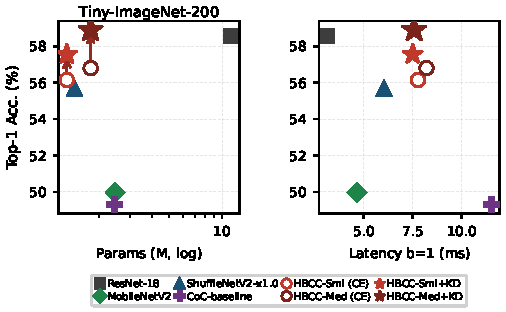
\includegraphics[width=\columnwidth]{pareto_tin}
  \caption{Pareto frontier trên Tiny-ImageNet-200. Mũi tên: mức
           tăng do KD. HBCC-Medium+KD~($\bigstar$) vượt ResNet-18
           trên cả hai trục với 6,26$\times$ ít tham số hơn.}
  \label{fig:paretotin}
\end{figure}

\begin{figure}[!t]
  \centering
  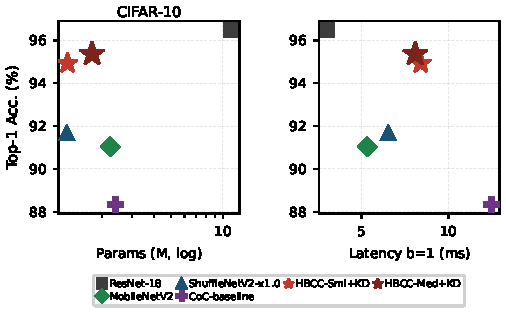
\includegraphics[width=\columnwidth]{pareto_cifar10}
  \caption{Pareto frontier trên CIFAR-10. HBCC+KD nằm ở vùng
           Pareto-dominant so với các baseline nhẹ trên cả trục tham
           số lẫn trục latency.}
  \label{fig:pareto10}
\end{figure}

\begin{figure}[ht!]
  \centering
  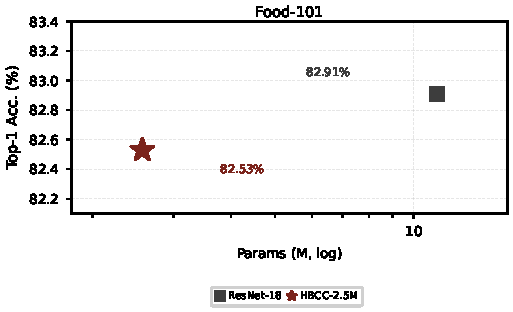
\includegraphics[width=\columnwidth]{pareto_food101}
  \caption{Phân bổ tham số trên Food-101 (chỉ trục tham số; độ trễ
           chưa được đo trong cùng điều kiện phần cứng ở độ phân giải
           $224\!\times\!224$). HBCC-2.5M~($\bigstar$) đạt 82,53\%
           với 4,38$\times$ ít tham số hơn ResNet-18.}
  \label{fig:paretofood}
\end{figure}

\subsubsection{Phân tích latency và bộ nhớ đỉnh}
\label{ssec:latency}

\noindent\textbf{Latency: ít MACs hơn nhưng vẫn chậm hơn.}
Mặc dù HBCC-Medium dùng ít MACs hơn ResNet-18 (138,9M vs 556,8M),
latency batch-1 lại cao hơn ($\approx\!8$~ms vs $\approx\!3$~ms) do
\textit{operator fragmentation}: ResNet-18 dành $\approx\!94\%$ thời
gian CUDA trong một kernel duy nhất (\texttt{cudnn\_convolution}),
trong khi HBCC phân tán trên nhiều kernel nhỏ (conv 1×1, bmm, vector
norm, scatter/gather). HBCC vẫn nhanh hơn CoC thuần $30$--$35\%$
(8\,ms vs 11\,ms).

\noindent\textbf{Bộ nhớ đỉnh: scatter buffer là nút cổ chai.}
HBCC-Medium đạt 481,6~MB (cao hơn ResNet-18 47\%) vì bước
scatter/gather phải đồng thời giữ tensor tương đồng và tổng đặc trưng
mỗi tầng; với \texttt{stem\_stride=1} các buffer lớn gấp $4\!\times$
so với CoC-baseline stride~2 (72,0~MB). Giảm \texttt{stem\_stride}
là đòn bẩy trực tiếp nhất.

\subsection{Thảo luận về tính phù hợp và hướng ứng dụng}
\label{sec:discussion}

\textbf{Kết quả tăng theo độ phức tạp không gian lớp.}
Trên CIFAR-10 (10 lớp), khoảng cách 1,12\% phản ánh độ lệch quy nạp
cục bộ của ResNet-18: đặc trưng cục bộ đã đủ khi không gian lớp đơn
giản, và khoảng cách đó đến từ mô hình có $6\times$ tham số hơn ---
hoàn toàn chấp nhận được. Trên Tiny-ImageNet-200 (200 lớp mịn), thứ
hạng đảo ngược: HBCC-Medium+KD vượt ResNet-18 giáo viên 0,32\% với
$6{,}26\!\times$ ít tham số hơn, xác nhận lợi thế ngữ cảnh tăng theo
độ phức tạp.

\textbf{Tại sao chưng cất tri thức đặc biệt hiệu quả trên bài toán
nhiều lớp mịn.}
Phân phối mềm ở nhiệt độ $T{=}4{,}0$ mã hóa mối quan hệ liên lớp:
các lớp ngữ nghĩa gần nhau (ví dụ: các giống chó, hoặc các dụng cụ
cùng hình dạng) nhận được xác suất dương trải đều từ giáo viên, cung
cấp tín hiệu học phong phú hơn nhãn one-hot. Cơ chế phân cụm ngữ cảnh
ở Tầng~3--4 tổng hợp thông tin không gian toàn cục thông qua gán và
tổng hợp có trọng số, phù hợp để hấp thu loại tín hiệu liên lớp này
hơn so với tích chập cục bộ, vốn xử lý các mảnh ảnh độc lập và thiếu
cơ chế mô hình hóa sự tương đồng toàn cục. Đây là lý giải cho việc
mức tăng KD trên Tiny-ImageNet-200 ($+$2,10\%/$+$1,41\%) lớn hơn so
với CIFAR-10 và đủ để học sinh vượt giáo viên trên tập kiểm tra.

\textbf{Hàm ý thiết kế từ thực nghiệm đối chiếu.}
Khoảng cách giữa HBCC và CoC-baseline mở rộng từ $+$7,02\% trên
CIFAR-10 lên $+$9,60\% trên Tiny-ImageNet-200, xác nhận giá trị của
nhánh cục bộ tăng theo độ phức tạp bài toán. LBPConv ở Tầng~1 mã hóa
kết cấu nhị phân không tham số; DWConv ở Tầng~2 tinh chỉnh thông tin
hình dạng cục bộ; cả hai cung cấp tín hiệu phân biệt không gian địa
phương mà phân cụm thuần không thể học được từ tổng hợp toàn cục.
Điều này gợi ý một nguyên tắc tổng quát: ở các tầng phân giải cao,
toán tử cục bộ tham số thấp mang lại tỉ lệ thông tin--chi phí tốt
hơn phân cụm toàn cục, và sự kết hợp bổ sung giữa hai loại trở nên
quan trọng hơn khi số lượng lớp tăng.

\textbf{Food-101: khả năng mở rộng và điểm cân bằng.}
Ở $224\!\times\!224$ với 101 lớp, khoảng cách thu hẹp còn 0,38\% top-1
với $4{,}38\!\times$ ít tham số hơn, cho thấy thiết kế lai mở rộng được
lên đầu vào độ phân giải chuẩn mà không đánh mất lợi thế tham số.
Trong bối cảnh này, HBCC và ResNet-18 đều chưa hội tụ trong 200
epoch (trạng thái tốt nhất của HBCC xuất hiện ở epoch cuối), gợi ý
rằng khoảng cách 0,38\% là giới hạn trên của khoảng cách thực sự và
có thể thu hẹp thêm với ngân sách huấn luyện lớn hơn.

\textbf{Khi nào HBCC phù hợp nhất.}
HBCC phù hợp nhất khi: (i)~không gian lớp rộng ($\gtrsim\!100$ lớp);
(ii)~độ phân giải đủ để tránh suy biến token;
(iii)~ngân sách tham số bị giới hạn nghiêm ngặt.
Với bài toán ít lớp không ràng buộc tài nguyên, CNN nhẹ chuẩn vẫn hiệu
quả hơn. Về ứng dụng thực tế, HBCC hướng đến các tình huống biên đòi
hỏi phân biệt nhiều lớp mịn --- nhận dạng món ăn, phân loại bệnh cây
trồng, giám sát loài động vật --- nơi tổng hợp ngữ cảnh và hiệu quả
tham số mang lại lợi ích lớn nhất.

\textbf{Hạn chế và hướng phát triển.}
Phân mảnh toán tử là thách thức thực tế chính: HBCC chạy chậm hơn
ResNet-18 dù ít MACs hơn vì các bước tổng hợp và phân phối dùng nhiều
kernel nhỏ không tối ưu trên GPU. Triển khai kernel CUDA hợp nhất
cho các bước này có thể rút ngắn latency đáng kể mà không thay đổi
kiến trúc. Bộ nhớ đỉnh cao do \texttt{stem\_stride=1} giữ bản đồ
đặc trưng $32\!\times\!32$ đến tận Tầng~1; stride thích ứng hoặc lượng
tử hóa tensor tương đồng là các hướng giảm thiểu tiềm năng. Biên nhỏ
trên Tiny-ImageNet-200 (0,32\,pp) và Food-101 (0,38\,pp) cần xác nhận
bằng nhiều seed độc lập. Hướng mở rộng tự nhiên bao gồm phát hiện đối
tượng và phân đoạn ngữ nghĩa, nơi tổng hợp ngữ cảnh toàn cục có thể
mang lại lợi ích lớn hơn phân loại ảnh.

% ============================================================
\section{Kết luận}
\label{sec:conclusion}

HBCC là kiến trúc lai bốn tầng áp dụng xử lý cục bộ (LBPConv,
DWConv) ở độ phân giải cao và phân cụm thuần ở độ phân giải thấp,
cùng stem stride~1 và fold giảm dần để khắc phục suy biến token.
HBCC-Medium+KD đạt \textbf{95,36\%} trên CIFAR-10 và \textbf{58,90\%}
trên Tiny-ImageNet-200 --- vượt ResNet-18 giáo viên với $6{,}26\!\times$
ít tham số hơn; HBCC-2.5M đạt \textbf{82,53\%} trên Food-101
($224\!\times\!224$) với $4{,}38\!\times$ ít tham số hơn ResNet-18.
Đặc biệt, việc học sinh 1,80M tham số vượt giáo viên 11,27M tham số
trên bài toán 200 lớp xác nhận rằng phân cụm ngữ cảnh khai thác
phân phối mềm của giáo viên hiệu quả hơn chính kiến trúc giáo viên
khi không gian lớp đủ phức tạp.

Kết quả xác nhận lợi thế của HBCC tăng theo độ phức tạp không gian
lớp --- không đáng kể trên CIFAR-10, rõ rệt trên Tiny-ImageNet-200,
cân bằng trên Food-101 --- cho thấy kiến trúc phù hợp nhất với nhận
dạng nhiều lớp mịn trong điều kiện tham số hạn chế. Ba nguyên tắc
thiết kế được xác lập: (i)~lựa chọn toán tử theo tầng khớp với độ
phân giải đặc trưng tối ưu hóa tỉ lệ thông tin--chi phí;
(ii)~fold giảm dần ngăn suy biến token mà không tốn thêm tham số;
(iii)~nhánh cục bộ tham số thấp cung cấp tín hiệu phân biệt không
gian địa phương mà phân cụm toàn cục thiếu, giá trị tăng khi số
lớp tăng.

Các hạn chế chính cần tiếp tục giải quyết: biên nhỏ trên
Tiny-ImageNet-200 (0,32\,pp) và Food-101 (0,38\,pp) cần xác nhận
đa seed; phân mảnh toán tử vẫn giữ latency và bộ nhớ cao hơn các
baseline tích chập có MACs tương đương; kết quả Food-101 phản ánh
hiệu năng kết hợp của kiến trúc và công thức huấn luyện, chưa tách
bạch từng yếu tố. Công việc tiếp theo sẽ tập trung vào tối ưu hóa
kernel CUDA để thu hẹp khoảng cách latency, chiến lược stride thích
ứng để giảm bộ nhớ đỉnh, và mở rộng đánh giá sang phát hiện đối
tượng và phân đoạn ngữ nghĩa.

% ============================================================

\bibliographystyle{IEEEtran}
\bibliography{references}

\end{document}
